% !TEX root = ../dg.tex

\section{Immersions and Embeddings}

Let's work up to proving \cref{thm:level set theorem}, including defining some more terminology.

\begin{definition}\label{def:immersion and embedding}
	Suppose $f \from M \to N$ is smooth. Then $f$ is an \emph{immersion} if $df_p$ is injective for all $p \in M$ (note that this implies $\dim(M) \leq \dim(N)$). 
	
	If $f$ is also a homeomorphism onto its image (continuous bijection with continuous inverse), then $f$ is an \emph{embedding}. The image of an embedding is a \emph{submanifold}. 
	
	If $f$ is bijective and $f^{-1}$ is smooth, then $f$ is a \emph{diffeomorphism}. $f$ is called a \emph{local diffeomorphism} at $p \in M$ if there exist neighborhoods $U$ of $p$ and $V$ of $f(p)$ so that $f \from U \to V$ is a diffeomorphism.
	
	Finally, we say that $f$ is a \emph{submersion} if $df_p$ is surjective for all $p \in M$.
\end{definition}

\begin{example}\label{ex:cusp}
	Define $\alpha \from \R \to \R^2$ by $\alpha(t) = (t^3, t^2)$ (see \cref{fig:cusp}).
	
	\begin{figure}[htbp]
		\centering
			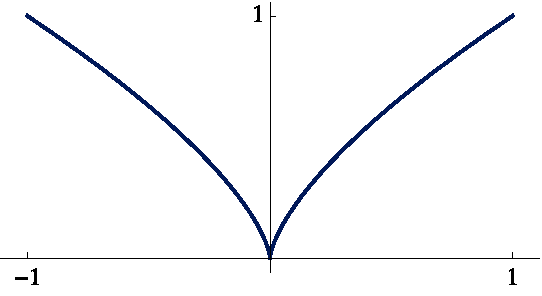
\includegraphics[height=1.5in]{cusp}
		\caption{The image of the map $\alpha$ from \cref{ex:cusp}. The fact that it has a cusp suggests that it will fail to be an immersion, despite being injective and smooth.}
		\label{fig:cusp}
	\end{figure}
	
	This is not an immersion because $d\alpha_0 = \begin{bmatrix} \alpha_1'(0) \\ \alpha_2'(0) \end{bmatrix} = \begin{bmatrix} 0 \\ 0 \end{bmatrix}$ has rank 0. Intuitively, the problem is that the velocity is zero when $t=0$, even though the map overall is continuous and injective.
\end{example}

\begin{example}\label{ex:conic}
	Define $\beta \from \R \to \R^2$ by $\beta(t) = (t^3 - 4t, t^2 - 4)$, which is a deformation of the previous example (see \cref{fig:conic}).
	
	\begin{figure}[htbp]
		\centering
			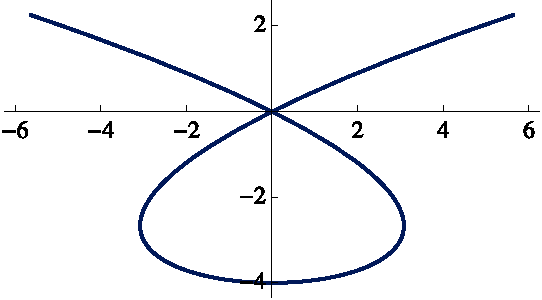
\includegraphics[height=1.5in]{conic}
		\caption{The image of the map $\beta$ from \cref{ex:conic}. This map is an immersion, but not an embedding.}
		\label{fig:conic}
	\end{figure}
	
	Now the differential is given by
	\[
		d\beta_t = \begin{bmatrix} 3t^2 - 4 \\ 2t \end{bmatrix},
	\]
	which is never the zero matrix since the second entry being 0 implies $t=0$, and hence that the first entry is $-4$. Hence, $d\beta_t$ is always rank 1, and hence always injective, so $\beta$ is an immersion.
	
	However, $\beta$ is not an embedding because it is not injective: $\beta(-2) = (0,0) = \beta(2)$, so there is a double point at the origin.
\end{example}

\begin{example}\label{ex:coordinate charts are local diffeomorphisms}
	Suppose $(U,\phi)$ is a local coordinate chart on a manifold $M$ containing a point $p \in M$. Then $\phi \from U \subset \R^n \to M$ is a local diffeomorphism at $\phi^{-1}(p) \in U$. This just follows from the definition of a coordinate chart (\cref{def:manifold}): $\phi$ maps $U$ bijectively onto $\phi(U)$, which is an open neighborhood of $p$, and both $\phi$ and $\phi^{-1}$ are smooth. (To be really pedantic, $(U, \operatorname{id})$ gives a global coordinate chart for the $n$-manifold $U$, and then, following \cref{def:differentiable}, $\phi \from U \to \phi(U)$ is smooth because $\phi^{-1} \circ \phi \circ \operatorname{id} = \operatorname{id}$ is smooth everywhere on $U$. Similarly, $\phi^{-1} \from \phi(U) \to U$ is smooth because $\operatorname{id} \circ \phi^{-1} \circ \phi = \operatorname{id}$ is smooth everywhere on $U$.)
\end{example}

If $f \from M \to N$ is a local diffeomorphism at $p \in M$, then $df_p \from T_pM \to T_{f(p)}N$ is a linear isomorphism (i.e., invertible linear map). Perhaps somewhat surprisingly, the converse is also true. This is the appropriate generalization of the Inverse Function Theorem to the manifold setting, and the proof essentially involves applying the Inverse Function Theorem in local coordinates:

\begin{proposition}\label{prop:local diffeomorphism}
	Suppose $f \from M \to N$ is smooth. If $p \in M$ and $df_p \from T_p M \to T_{f(p)}N$ is an isomorphism, then $f$ is a local diffeomorphism at $p$.
\end{proposition}

\begin{proof}
	We are going to apply the Inverse Function Theorem (\cref{thm:inverse function theorem} below) to $\psi^{-1} \circ f \circ \phi \from \phi(U) \to \psi(V)$, where $(U,\phi)$ and $(V, \psi)$ are the coordinate charts guaranteed to exist by the definition of smoothness (\cref{def:differentiable}).
	
	Notice that, by the Chain Rule,
	\[
		d(\psi^{-1} \circ f \circ \phi)_{\phi^{-1}(p)} = d\psi^{-1}_{f(p)} \circ df_p \circ d\phi_{\phi^{-1}(p)}.
	\]
	But then we already know that $d\phi$ and $d\psi^{-1}$ are isomorphisms (since coordinate charts are local diffeomorphisms [\cref{ex:coordinate charts are local diffeomorphisms}]), so $df_p$ being an isomorphism implies that $d(\psi^{-1} \circ f \circ \phi)_{\phi^{-1}(p)}$ is also an isomorphism.
	
	But then the Inverse Function Theorem implies $\psi^{-1} \circ f \circ \phi$ is a local diffeomorphism at $\phi^{-1}(p)$. Since $\psi$ and $\phi^{-1}$ are local diffeomorphisms (again, \cref{ex:coordinate charts are local diffeomorphisms}) and compositions of local diffeomorphisms are local diffeomorphisms, it follows that
	\[
		\psi \circ (\psi^{-1} \circ f \circ \phi) \circ \phi^{-1} = (\psi \circ \psi^{-1}) \circ f \circ (\phi \circ \phi^{-1}) = f
	\]
	is also a local diffeomorphism.
\end{proof}

Here's a statement of the Inverse Function Theorem in the language of differentials and local diffeomorphisms. It is equivalent to the usual statement you would see in a multivariable calculus or analysis course.

\begin{exercise}
	Convince yourself of the previous sentence.
\end{exercise}

\begin{theorem}[Inverse Function Theorem]\label{thm:inverse function theorem}
	If $F \from U \subseteq \R^n \to \R^n$ is given by $(x_1, \dots , x_n) \mapsto (y_1, \dots , y_n)$, then $dF_p = \begin{bmatrix} \left.\frac{\partial y_i}{\partial x_j}\right|_p\end{bmatrix}_{i,j}$ being nonsingular at $p \in U$ implies that $F$ is a local diffeomorphism at $p$.
\end{theorem}

We're now ready to prove the Level Set Theorem (\cref{thm:level set theorem}):

\begin{proof}[Proof of \cref{thm:level set theorem}]
	Recall that, in the statement, we're assuming that $f\from M \to N$ is smooth and that $q \in N$ is a regular value of $f$, and the goal is to show that $f^{-1}(q)$ is a smooth submanifold of $M$ of dimension $m-n$.
	
	Suppose $(U,\phi)$ is a coordinate chart centered at $p \in f^{-1}(q)$\footnote{Meaning that $p = \phi(\vec{0})$.} and $(V, \psi)$ is a chart at $q$. See \cref{fig:level set theorem}. Then define the map
	\[
		g := \psi^{-1} \circ f \circ \phi: U \to \R^n.
	\]
	By assumption,
	\[
		dg_{\vec{0}} = d(\psi^{-1} \circ f \circ \phi)_{\vec{0}} = (d \psi^{-1})_{f(p)} \circ df_p \circ d\phi_{\vec{0}}
	\]
	is surjective since $df_p$ is and the other two terms are isomorphisms.
	
	\begin{figure}[htbp]
		\centering
			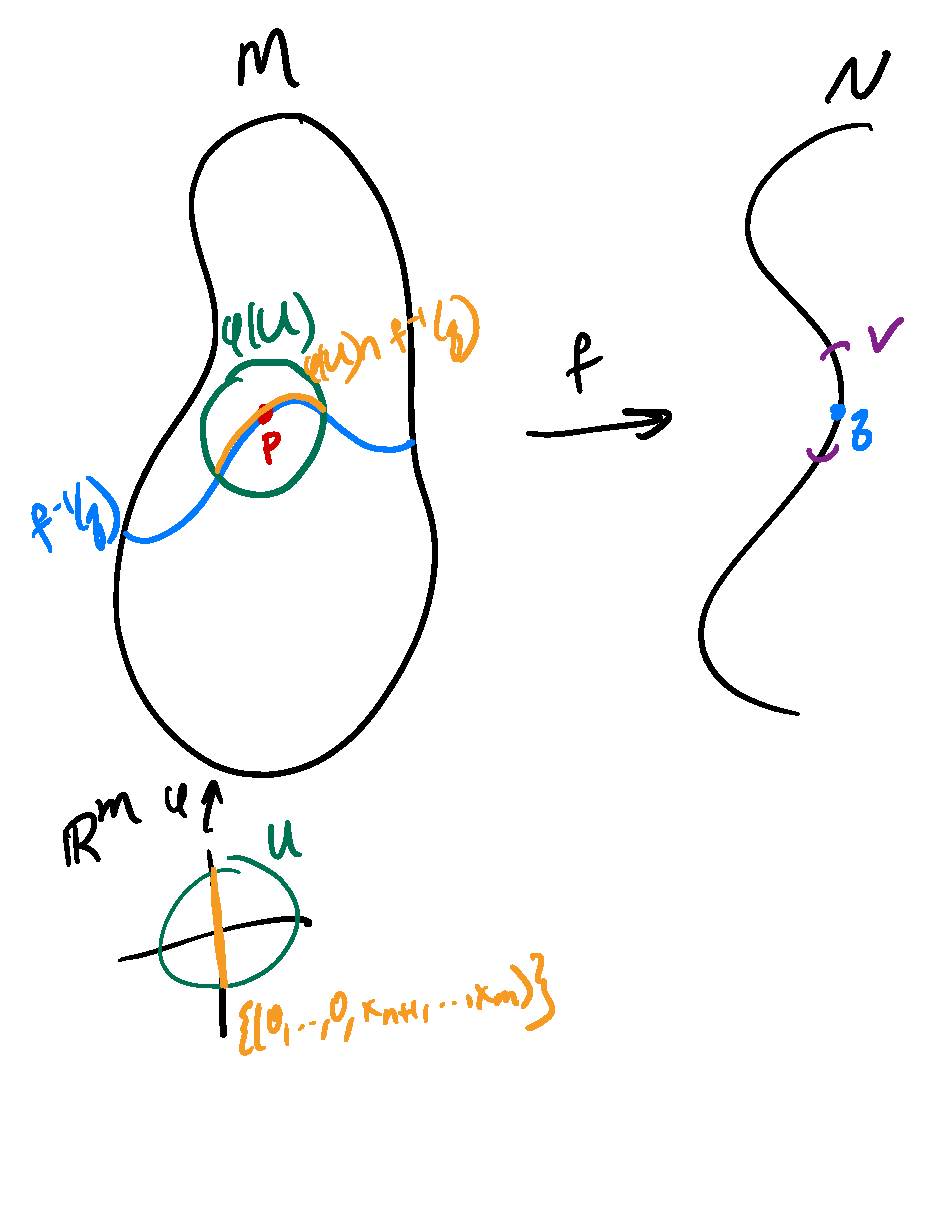
\includegraphics[height=2.5in]{level-set-theorem}
		\caption{A sketch of the key neighborhoods and maps in the proof of \cref{thm:level set theorem}.}
		\label{fig:level set theorem}
	\end{figure}
	
	Hence, after a linear change of coordinates $dg_{\vec{0}}$ can be written as the $n \times m$ block matrix $\begin{bmatrix} I_{n \times n} & 0_{n \times (m-n)} \end{bmatrix}$. Define
	\[
		G(x_1, \dots , x_m) = (g(x_1, \dots , x_n), x_{n+1}, \dots , x_m),
	\]
	which has differential $dG_{\vec{0}} = I_{m \times m}$ in these coordinates. By the Inverse Function Theorem, $G$ is a local diffeomorphism at $\vec{0}$ and by construction $g \circ G^{-1}$ is the standard projection onto the first $n$ coordinates.
	
	So in these coordinates $f^{-1}(q) \cap \phi(U) = \phi(0, \dots , 0, x_{n+1}, \dots , x_m)$, so $x_{n+1} , \dots , x_m$ give local coordinates near $p$ for $f^{-1}(q)$. We can do the same at any other point of $f^{-1}(q)$, so this gives a system of coordinate charts on $f^{-1}(q)$, and the transition maps on overlapping charts are smooth because they are just restrictions (or projections, if you prefer) of the corresponding transition maps for the charts on $M$.
\end{proof}